\begin{frame}{Formalisation de l'approche}
	\begin{itemize}
%		\item extraction terminologique
		\item comparaison des résultats avec la liste des concepts (vérité terrain)
%				\item prise en compte des synonymes des termes
%		\begin{itemize}
%			\item ex. \textit{paralysie agitante} $\rightarrow$ \textit{maladie de Parkinson} 
%		\end{itemize}
		\item recenser le score le plus élevé sur le terme ou sur son synonyme
	\end{itemize}
	\begin{figure}[h]
		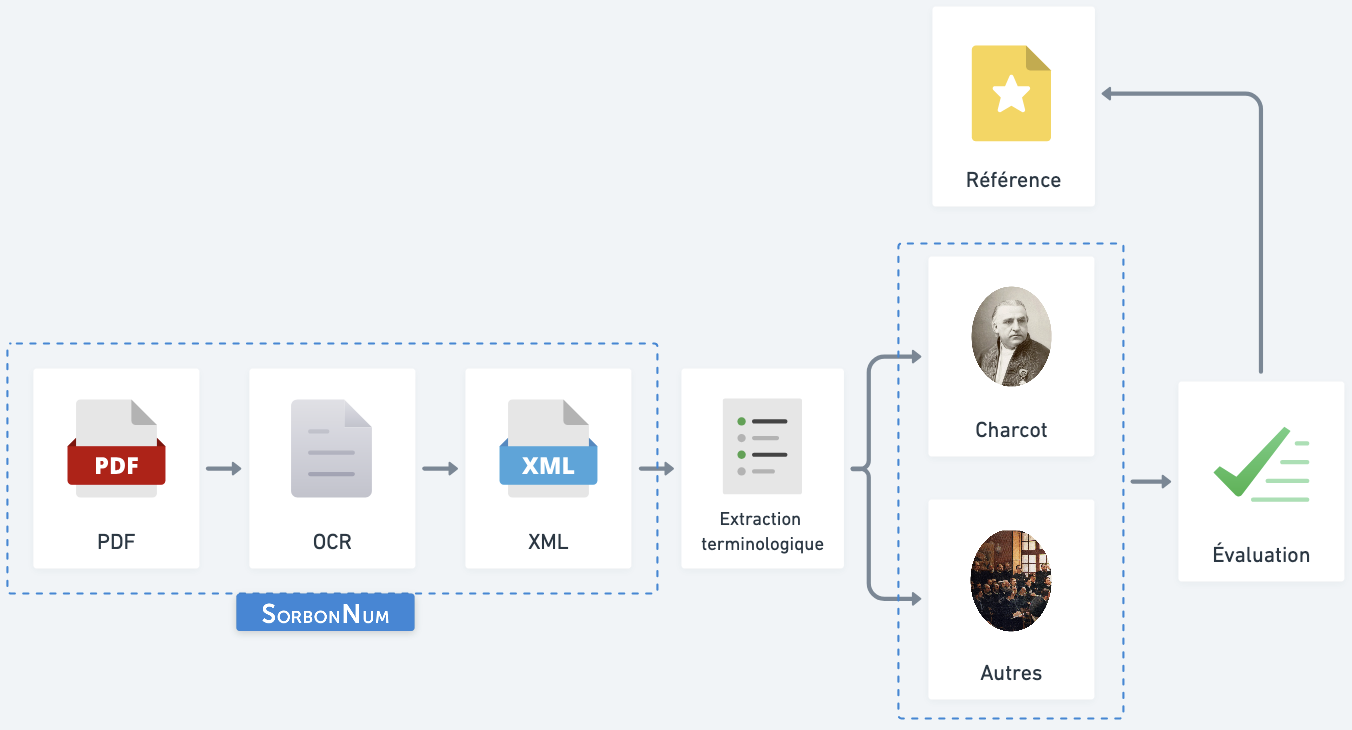
\includegraphics[width=\linewidth]{pic/formalisation_approche.png}
		\caption{\textit{Pipeline} pour pister la circulation des termes médicaux associés à Charcot.}
		\label{fig:ling_out_TAL}
	\end{figure}
\end{frame}

\begin{frame}{Liste des concepts médicaux -- vérité terrain}
	Extraction semi-automatique des termes en lien avec Charcot.\\{\scriptsize\url{https://github.com/ljpetkovic/Charcot\_circulations/tree/main/concepts}}
	
	\begin{figure}[!htb]
		\centering
		\begin{minipage}{.5\textwidth}
			\centering
			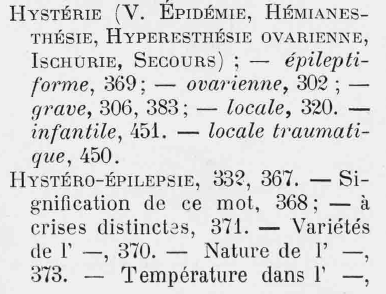
\includegraphics[width=0.6\linewidth, height=0.3\textheight]{pic/concepts-pdf}
			\caption{Index des termes \parencite{charcot1892oeuvres}.}
			\label{fig:prob1_6_2}
		\end{minipage}%
		\begin{minipage}{.5\textwidth}
			\centering
			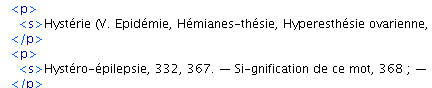
\includegraphics[width=1\linewidth, height=0.15\textheight]{pic/concepts-xml}
			\caption{Concepts médicaux, document XML.}
			\label{fig:prob1_6_1}
		\end{minipage}
	\end{figure}
	\begin{figure}[!htb]
		\centering
		\begin{minipage}{.5\textwidth}
			\centering
			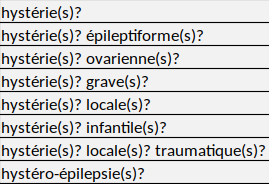
\includegraphics[width=0.6\linewidth, height=0.25\textheight]{pic/concepts-csv}
			\caption{Liste finale des concepts médicaux.}
			\label{fig:prob1_6_2}
		\end{minipage}%
		\begin{minipage}{.6\textwidth}
			\centering
			\begin{enumerate}
				\setcounter{enumi}{0}
				\item entre \texttt{<s>} et \texttt{,-(} (regex)
				\item sans termes génériques (\textit{os}, \textit{peau})
				\item prise en compte des sg. / pl. (regex)
			\end{enumerate}
		\end{minipage}
	\end{figure}
\end{frame}

